% 
% topic Template for ME3023 - Measurements in Mechanincal Systems - Tennessee Technological University
%
% Spring 2020 - Summer 2020
% Tristan Hill, May 31, 2020
% Introduction - Topic 2 - Types of Variables
% 

%\documentclass{beamer}                         % for presentation (has nav buttons at bottom)
\documentclass[handout]{beamer}  % for handout 
\usepackage{beamerthemesplit}
\usepackage{amsmath}
\usepackage{listings}
\usepackage{multicol}
\usepackage{framed}

\beamertemplateballitem

\definecolor{TTUpurple}{rgb}{0.3098, 0.1607, 0.5176} % TTU Purple (primary)
\definecolor{TTUgold}{rgb}{1.0000, 0.8666, 0.0000} % TTU Gold (primary)

\setbeamercolor{palette primary}{bg=TTUpurple,fg=TTUgold}
\setbeamercolor{palette secondary}{bg=black,fg=TTUgold}
\setbeamercolor{palette tertiary}{bg=black,fg=TTUpurple}
\setbeamercolor{palette quaternary}{bg=TTUgold,fg=black}
\setbeamercolor{structure}{fg=TTUpurple} % itemize, enumerate, etc
\setbeamercolor{section in toc}{fg=TTUpurple} % TOC sections

% custom colors 
\definecolor{mygray}{rgb}{.6, .6, .6}
\definecolor{mypurple}{rgb}{0.6,0.1961,0.8}
\definecolor{mybrown}{rgb}{0.5451,0.2706,0.0745}
\definecolor{mygreen}{rgb}{0, .39, 0}

% color commands
\newcommand{\OR}{\color{orange}}
\newcommand{\R}{\color{red}}
\newcommand{\B}{\color{blue}}
\newcommand{\BR}{\color{mybrown}}
\newcommand{\K}{\color{black}}
\newcommand{\G}{\color{mygreen}}
\newcommand{\PR}{\color{mypurple}}
%\usefonttheme{professionalfonts}

\newcommand{\Lagr}{\mathcal{L}} % lagrangian

\newcommand{\vspccc}{\vspace{6mm}\\} % large vertical space
\newcommand{\vspcc}{\vspace{4mm}\\}   % medium vertical space
\newcommand{\vspc}{\vspace{2mm}\\}     % small vertical space

\newcommand{\hspcccc}{\hspace{10mm}} % large horizontal space
\newcommand{\hspccc}{\hspace{6mm}} % large horizontal space
\newcommand{\hspcc}{\hspace{4mm}}   % medium horizontal space
\newcommand{\hspc}{\hspace{2mm}}     % small horizontal space

\author{ME3023 - Measurements in Mechanical Systems} % original formatting from Mike Renfro, September 21, 2004

\newcommand{\MNUM}{1\hspace{2mm}} % Module number
\newcommand{\TNUM}{2\hspace{2mm}} % Topic number 
\newcommand{\moduletitle}{Introduction }
\newcommand{\topictitle}{Types of Variables } 

\title{Module \MNUM - \moduletitle}

\date{May 29, 2020}

\begin{document}

\lstset{language=MATLAB,basicstyle=\ttfamily\small,showstringspaces=false}

\frame{\titlepage \center\begin{framed}\Large \textbf{Topic \TNUM - \topictitle}\end{framed} \vspace{5mm}}

% Section 0: Outline

\frame{

\large \textbf{Topic \TNUM - \topictitle} \vspace{3mm}\\

\begin{itemize}
	\item Measured Variable \vspc % Section 1
	\item Independent and Dependent Variables  \vspc % Section 2
	\item Controlled Variables and Parameters  \vspc % Section 3
	\item Extraneous Variables  \vspc % Section 3
	\item Engineering Example   \vspc % Section 4
\end{itemize}

}

% Section 1
\section{Measured Variable}
\frame{
\frametitle{Measured Variable}

\large{``A {\B measurement} is an act of assigning a specific value to a physical variable. That physical variable
is}\vspc% the {\G measured variable}.''} \vspc
{\tiny Text: Theory and Design of Mech. Meas.}

}

% Section 2
\section{Independent and Dependent Variables}
\frame{
\frametitle{Independent and Dependent Variables}

{``If a change in one variable will not affect the value of some other variable, the
two are considered independent of each other. A variable that can be changed independently of other
variables is known as an \underline{\hspace{30mm}} \underline{\hspace{30mm}}. A variable that is affected by changes in one or more other variables is known as a  \underline{\hspace{30mm}} \underline{\hspace{30mm}}. Normally, the variable that we measure depends on }\vspace{10mm}\\
{\tiny Text: Theory and Design of Mech. Meas.}

}

% Section 3
\section{Controlled Variable}
\frame{
\frametitle{Controlled Variables and Parameters}

{``A variable is \underline{\hspace{30mm}} if it can be held at a constant value
or at some prescribed condition during a measurement... ...complete control of a variable is not usually
possible. We use the adjective\underline{\hspace{30mm}} to refer to a variable that can be held as prescribed, at
least in a nominal sense... \vspc
...we define a \underline{\hspace{30mm}} as a functional grouping of variables. For example, a moment of inertia or a Reynolds number... ...A \underline{\hspace{30mm}} that has an effect on the behavior of the measured variable is called a control parameter....''} \vspc
{\tiny Text: Theory and Design of Mech. Meas.}

}

% Section 4
\section{Extraneous Variables}
\frame{
\frametitle{Extraneous Variables}

{``Variables that are not or cannot be controlled during measurement but that affect the value of the
variable measured are called \underline{\hspace{30mm}} \underline{\hspace{30mm}}. Their influence can confuse the clear relation
between cause and effect in a measurement... ...The effects due to \underline{\hspace{30mm}} \underline{\hspace{30mm}} can take the form of signals superimposed
onto the measured signal with such forms as {\PR noise} and drift.''} \vspc
{\tiny Text: Theory and Design of Mech. Meas.}

}
% Section 5
\section{Engineering Example}
\frame{
\frametitle{Engineering Example}


	\textbf{ SHARP I.R. Ranger - Distance Sensor} \vspc
	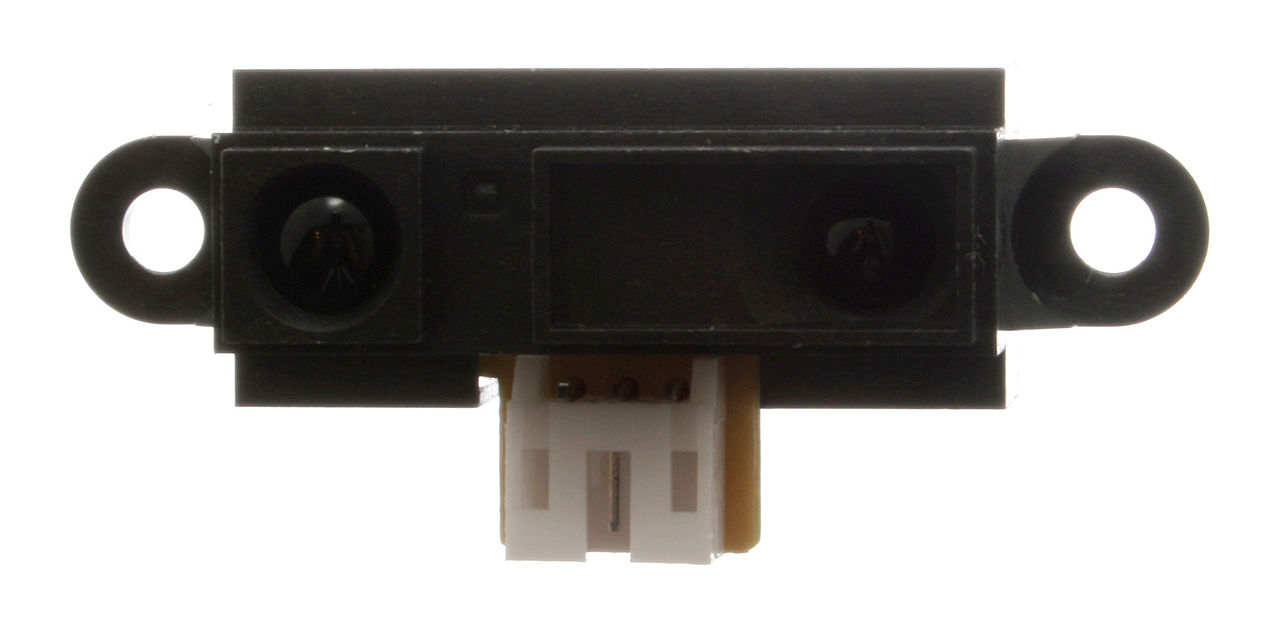
\includegraphics[scale=0.5]{proximity_sensor.jpg} \hspace{20mm}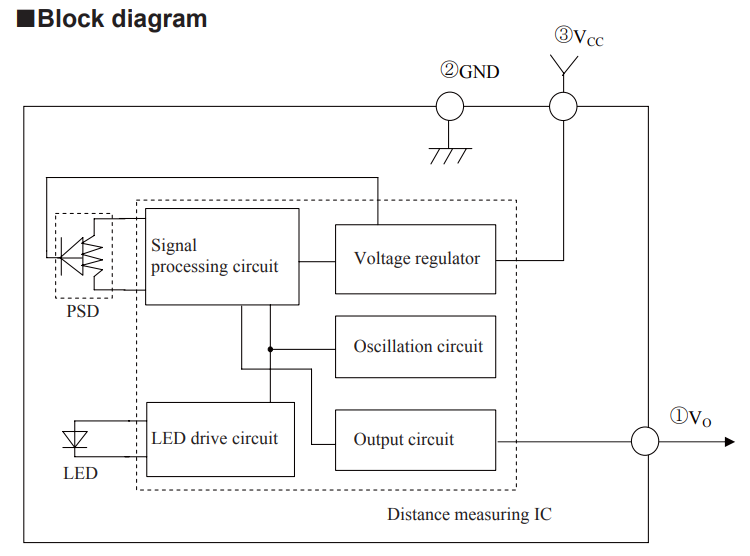
\includegraphics[scale=0.20]{sharp_ranger_circuit.png} \vspc
  {\tiny Image, More Info: \href{https://en.wikipedia.org/wiki/Proximity_sensor}{Wikipedia} }\hspace{40mm} {\tiny Image, More Info: \href{https://en.wikipedia.org/wiki/Position_sensitive_device}{Wikipedia} }

}

\frame{
\frametitle{Engineering Example}


Consider the IR distance ranger, name at least one physical variable for each of the following categories. 

\begin{itemize}
	\item Measured Variable \vspc 
	\item Independent Variable \vspc
	\item Dependent Variables  \vspc 
	\item Controlled Variables  \vspc 
	\item Extraneous Variables  \vspc 
\end{itemize}

}

\end{document}





